\documentclass{LabReport}
\title{计算方法数值实验1-实验报告}
\author{221900180 田永铭}
\date{\today}
\addbibresource{refs.bib}
\Chead{计算方法数值实验1-实验报告 221900180 田永铭}
\Cfoot{\thepage}
\usepackage{listings}
\usepackage{graphicx} 
\usepackage{tikzsymbols}
\usepackage{tikz}
\usepackage{hyperref}

\begin{document}
	\maketitle
	
	\section{实验题目}
利用matlab实现复化梯形公式、复化Simpson公式、Romberg加速算法,并将算法应用到求解三个数值积分上。需要输出数值结果、等分区间数、下三角输出(Romberg算法),误差取为1e-7。数值积分如下:
$1.I1 = \int_{0.1}^{4}\frac{sinx}{x} dx\quad$$2.I2 = \int_{-2}^{4}e^{-x^2} dx\quad$$3.I3 = \int_{0}^{1}\frac{ln(1+x)}{x} dx$


	\section{实验原理及相关说明}
	\begin{itemize}
		\item \textbf{实验原理:}复化梯形公式和复化Simpson公式都是通过等分节点插值型求积公式推导出来的求积公式,而Romberg算法利用二分区间前后的截断误差的关系,推导出了一种建立T数表的更快的求积方法,有良好的性质。
		\item \textbf{相关说明1——实验环境和作业独立性:}本人此次实验全部采用matlab实现,全程独立实现无参考。
		\item \textbf{相关说明2——关于方法的说明:}主要根据书上公式来一一实现,特别要注意第三个积分要单独处理0处的数值。梯形和simpson公式的分点我按照2的幂次来取,误差通过误差公式来求二阶或者四阶导函数的最大值来估计,从而区间数依从取1,2,4,8...直到满足精度要求(实际可能要取得点更少,我取这么多一定能够保证)。Romberg的误差直接使用公式即可。
		\item \textbf{相关说明3——关于结果的说明:}关于结果的说明:
		结果均保证了误差在1e-7以内且三种方法高度统一。与matlab直接调用integral积分函数得出的结果在精度范围内完全一致。
	\end{itemize}
	
	\section{核心代码以及注释说明}
	\subsection{复化梯形公式}
	
\begin{lstlisting}[language=python,frame=shadowbox]
a = 0.1	;b = 4;	acc = 1e-7; % 积分1
syms x;	f = @(x)sin(x)/x;  % 定义函数

% 计算函数导数的值并找到最大值方便后面误差判断
df = diff(f,x,2); df = matlabFunction(df);
xx = linspace(a,b,1000); yy = zeros(size(xx));
for i = 1:length(xx)
	yy(i) = double(df(xx(i)));
end
max_value = max(yy);

%调用复合梯形公式,结果打包成display返回
[y,n,points] = trapezoid(f, a, b, acc,max_value);
display = [y,n,points];


function [y,n,points] = trapezoid(f, a, b, acc,max_value)
n = 1; %区间数字	points = n + 1; %区间点数
y = (b-a)/2*(f(a)+f(b));%梯形公式求初值
err = b-a;%初始误差

while err >= acc
	n = n * 2; %二分
	h = (b-a)/n; 
	Sigma = 0;
	for k = 1:(n-1)
		Sigma = Sigma + f(a + k*h);
	end
	y = (h/2)*(f(a)+f(b)+2*Sigma);
	err = abs((b-a)/12*h*h*max_value) ; %复化梯形公式
end
	points = n + 1; %更新点数
	return
end
\end{lstlisting}

\subsection{复化Simpson公式}
\begin{lstlisting}[language=python,frame=shadowbox]
% 略去和复化梯形公式完全类似的部分,注意用四阶导最大值表示误差
% 以下为核心公式部分:
while err >= acc
	n = n * 2;
	h = (b-a)/n;
	Sigma = 0;
	for k = 1:(n-1)
		Sigma = Sigma + f(a + k*h);
	end
	Sigma2 = 0;
	for k = 0:(n-1)
		Sigma2 = Sigma2 + f(a + (k+1/2)*h);
	end
	y = (h/6)*(f(a)+f(b)+2*Sigma+4*Sigma2);
	err = abs((b-a)/180*h*h*h*h/2/2/2/2*max_value) ;
	end
\end{lstlisting}

{\color{red} 对这两个公式的说明:}我采用的是两种公式的初始的积分余项来估算误差,另一种方式是利用二分前后截断误差的关系来近似误差,这两种方式都行。不过,这都是能保证了精度要求 ,当然也可能不需要这么多区间就已经能达到精度要求。所以{\color{red} 区间可能略大,}但是不影响结果。

\subsection{Romberg加速算法}
\begin{lstlisting}[language=python,frame=shadowbox]
function y = Romberg(f, a, b, acc)
k = 0;	%目前更新到的行数
T = zeros(10,10,'double'); % 定义T数表
T(1,1) = (b-a)/2*(f(a)+f(b)); %梯形公式求出T(0,0)
err = b-a; 初始误差

while err >= acc
	k = k+1; %一个循环更新一行
	Sigma = 0;
	for i = 1:pow2(k-1)
		Sigma = Sigma + f(a+(2*i-1)*(b-a)/pow2(k) );
	end
	T(1,k+1) = (1/2)*(T(1,k)+(b-a)/pow2(k-1) * Sigma ); 

	for j=1:k
		T(j+1,k-j+1) = (power(4,j)*T(j,k-j+1+1)-T(j,k-j+1))
		/(power(4,j)-1);
	end
	%误差公式为 T(k,0)和T(k-1,0)的差值的绝对值
	err= abs(T(k+1,1)-T(k,1));
	y = T(k+1,1);
end
	return
end
\end{lstlisting}

{\color{red} 对Romberg算法的说明:}由于matlab中的矩阵下标从1开始定义而不是从0开始,所以下标略有区别。按照求T数表的公式来求解T的值,按照误差公式判断结束即可。

\section{实验结果}

\subsection{复化梯形公式}	
\begin{figure}[h!]
	\centering
	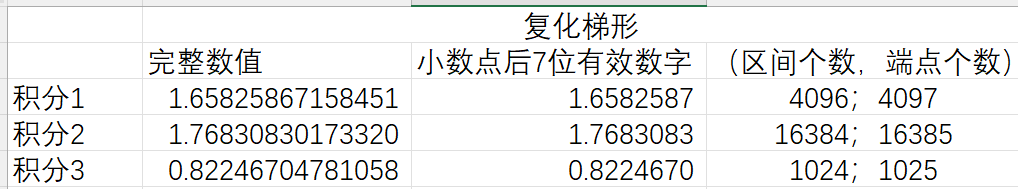
\includegraphics[width=0.7\linewidth]{figures/1}
	\label{fig:1}
\end{figure}


\subsection{复化Simpson公式}
\begin{figure}[h!]
	\centering
	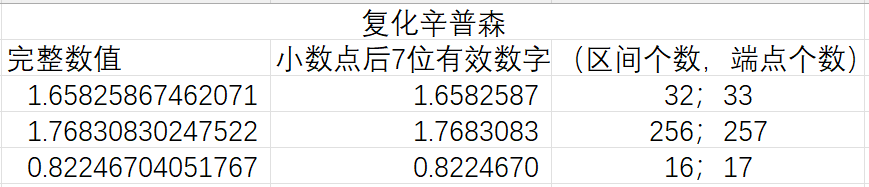
\includegraphics[width=0.7\linewidth]{figures/2}
	\label{fig:2}
\end{figure}

\subsection{Romberg加速算法}

\begin{figure}[h!]
	\centering
	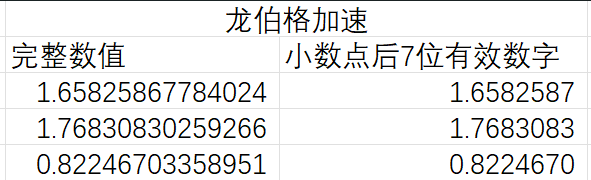
\includegraphics[width=0.7\linewidth]{figures/3}
	\caption{计算结果}
	\label{fig:3}
\end{figure}

\begin{figure}[h!]
	\centering
	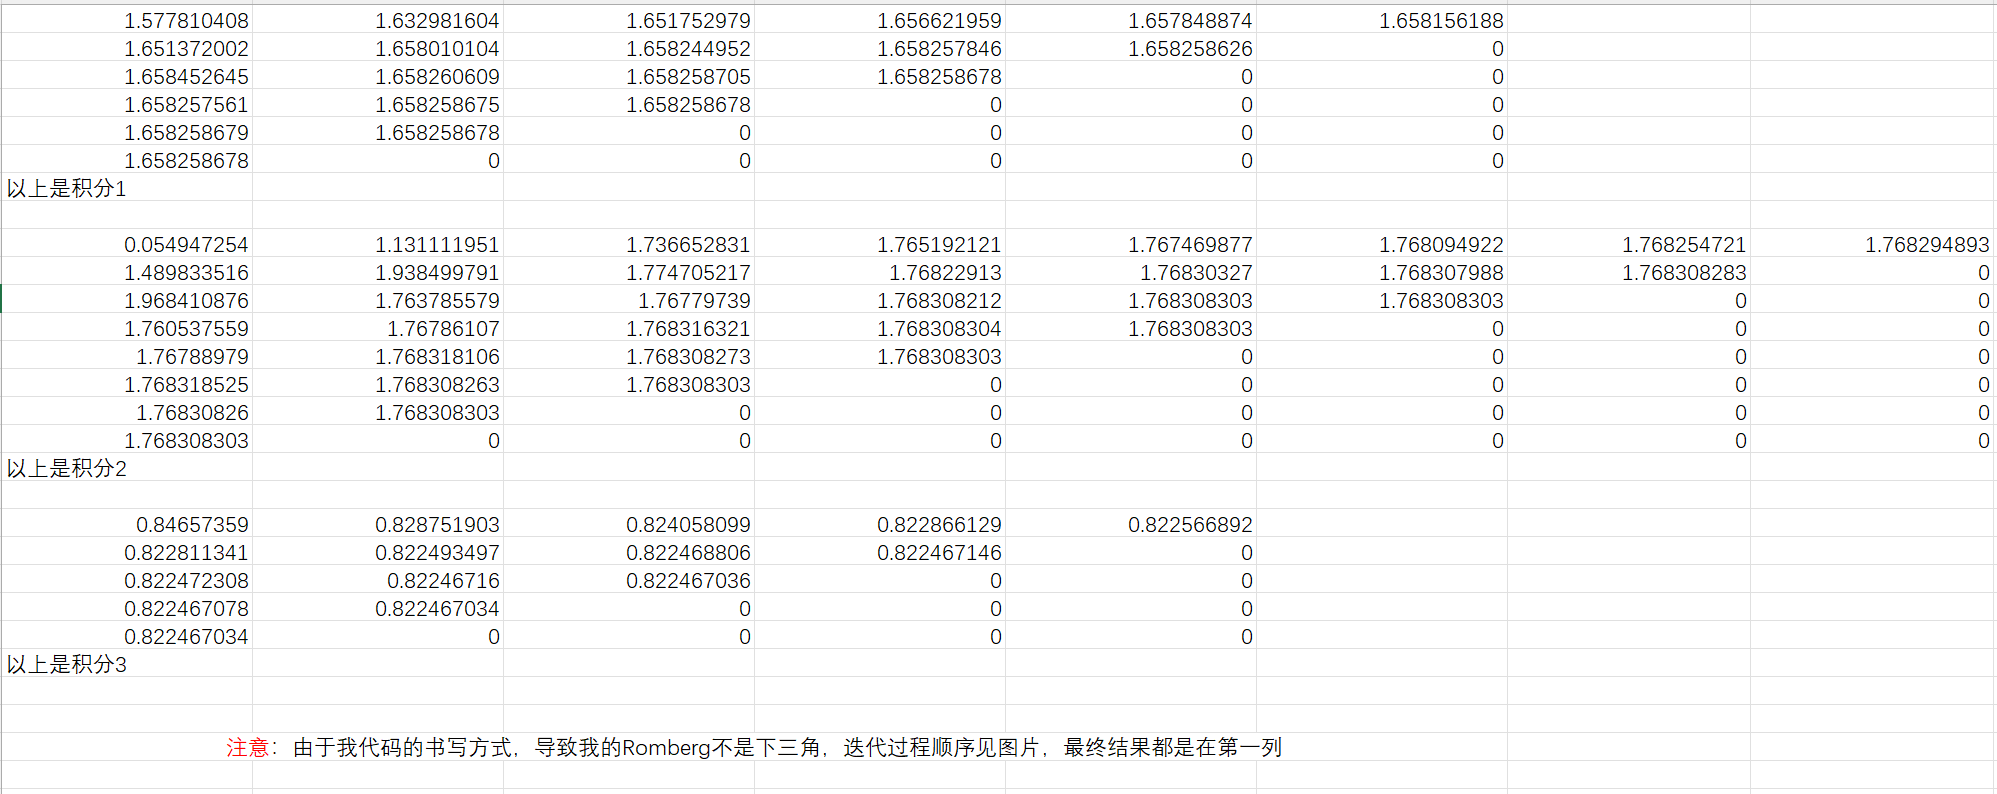
\includegraphics[width=1\linewidth]{figures/4}
	\caption{T数表结果(分别顺序对应三个积分)}
	\label{fig:4}
\end{figure}

\begin{figure}[h!]
	\centering
	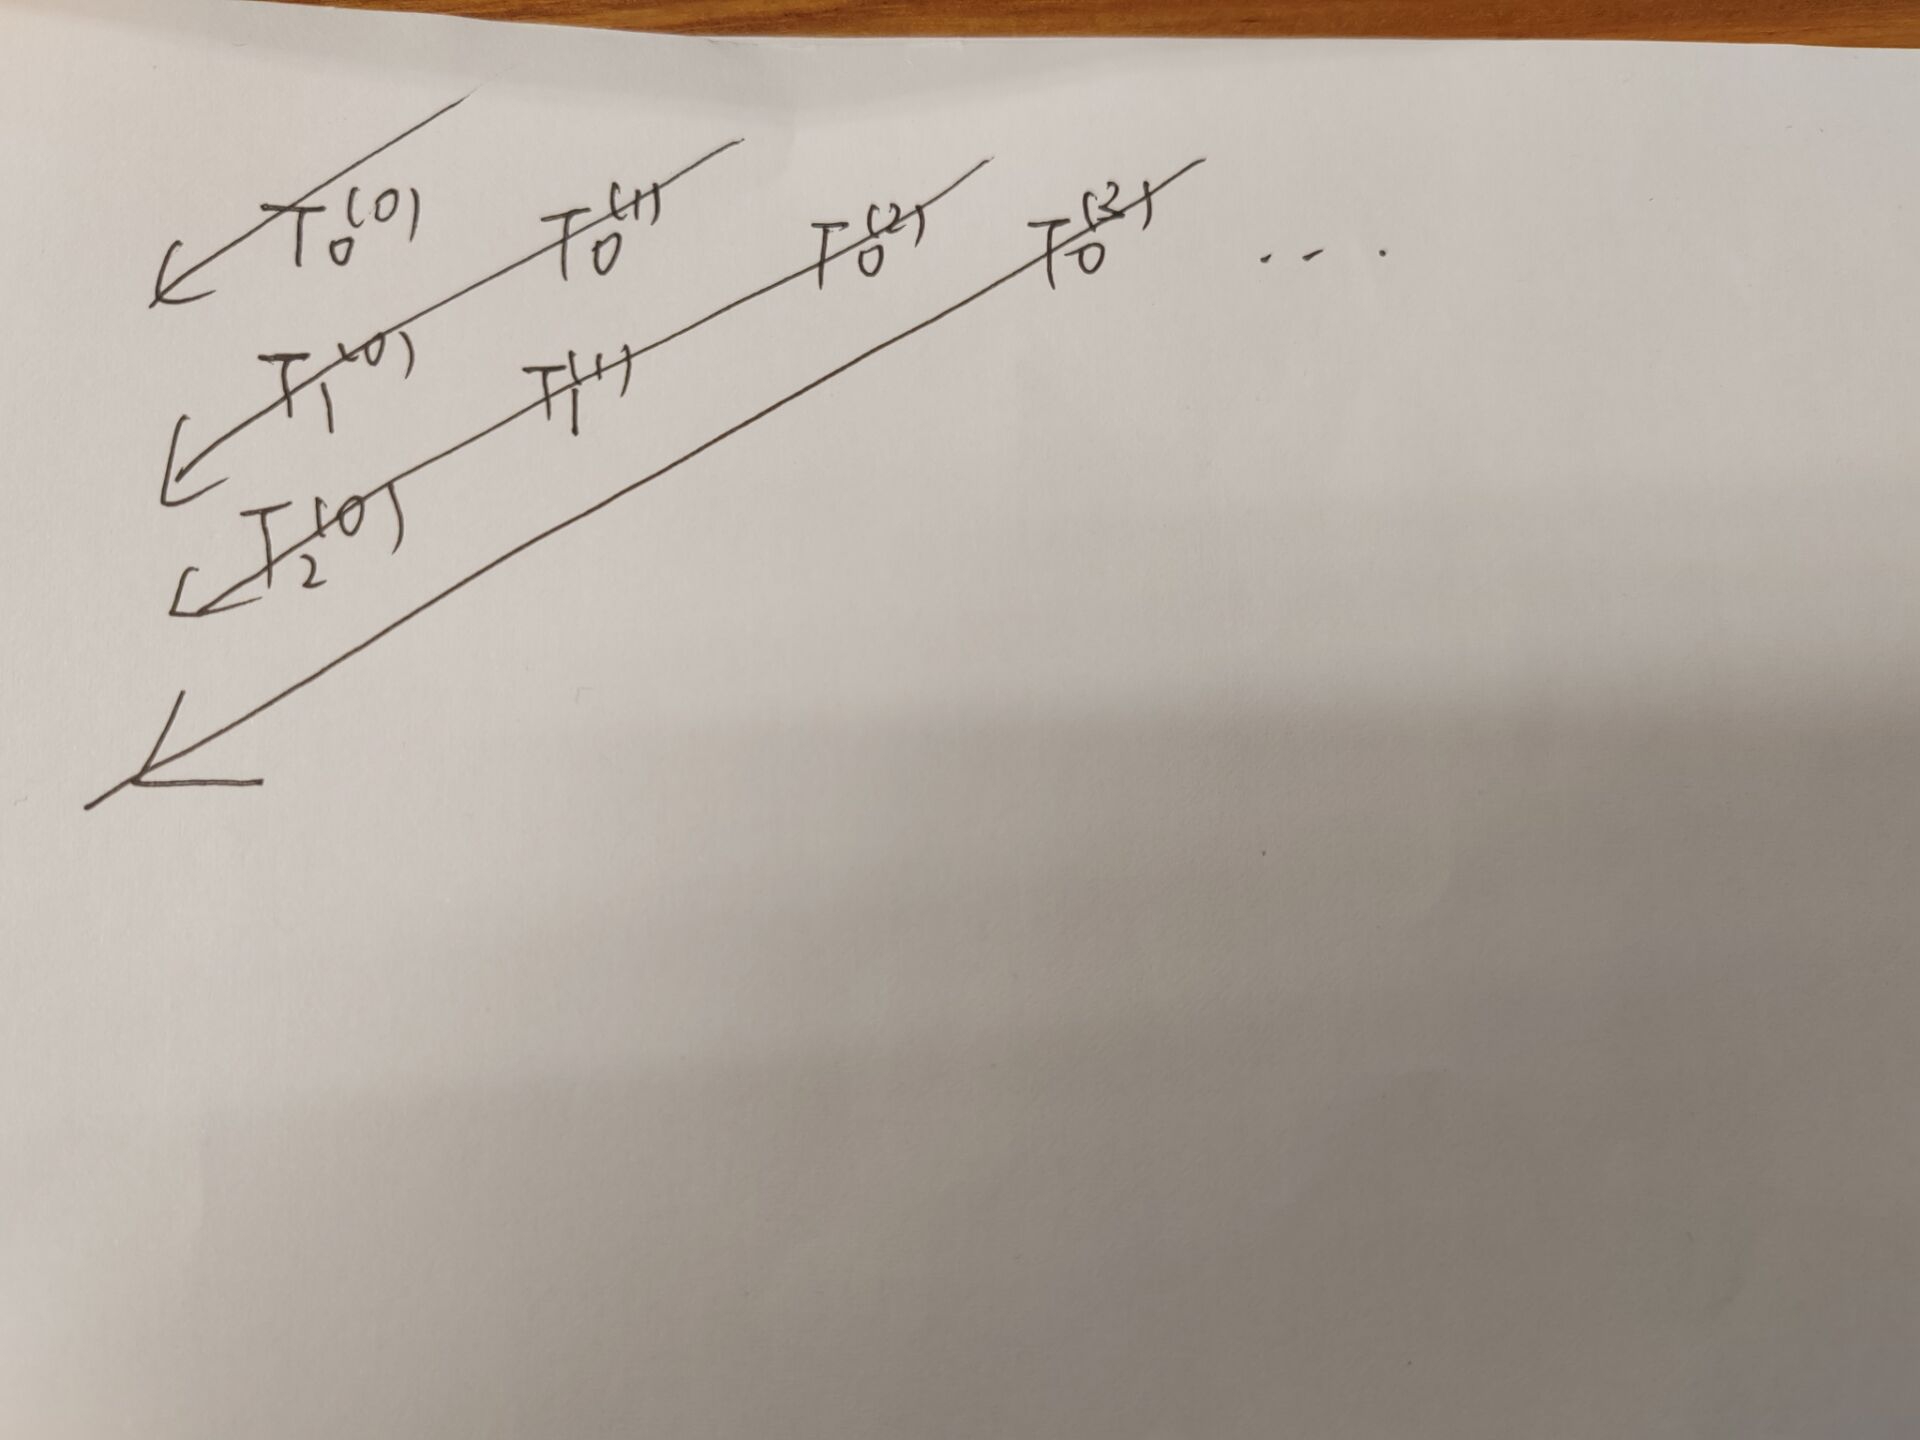
\includegraphics[width=0.7\linewidth]{figures/5}
	\caption{T数表结构}
	\label{fig:5}
\end{figure}

{\color{red} 对结果的说明:}三种结果都保证了达到小数点后7位有效数字,且计算结果完全统一。相比之下,三种方法中复化梯形方法所需的等分节点最多,复化Simpson方法较少,而Romberg方法是一种收敛速度极快的算法。T数表的结构这里没用下三角,形成的是另外一种三角,但是实质是一样的。结果完全符合预期。

\section{总结}

\begin{enumerate}
	\item 通过这次实验,我对复化梯形公式、复化Simpson公式、Romberg加速算法的理解更深了一步,理解了算法的原理、收敛速度、注意点和操作细节等等。
	\item 我主动选择了使用matlab这个之前未使用过的工具,了解了它的基础使用方法,并利用它完成了数值实验。正如老师所说,这是一款数学上的很好的工具。
	\item 通过这次实验,我理论联系实际,将书本知识应用到程序上,激发了对计算方法这门课程的极大的兴趣。同时也明白了,数值实验是有误差的,是``差不多"的,但是做实验必须是仔细和精确到每一个细节的,例如第三个积分的0处值的处理等等。
\end{enumerate}

\end{document}
